\chapter{Agrupamiento jerárquico}


El clustering jerárquico es un algoritmo de aprendizaje no supervisado, agrupa los  datos en jerarquía y de allí su nombre. La jerarquía se representa a través de un dendrograma o árbol que muestra las relaciones de inclusión de los diferentes
grupos. Dentro del clustering jerárquico tenemos dos grandes enfoques:

\begin{itemize}
    \item \textit{Clustering} jerárquico aglomerativo o \textit{bottom-up}.

    \item \textit{Clustering} jerárquico divisivo o \textit{top-down}.
\end{itemize}

\section{Clustering jerárquico aglomerativo o bottom-up}

Se denomina aglomerativo porque empieza con grupos muy pequeños hasta formar  un grupo. En este caso, cada punto del conjunto de datos comienza como un clúster individual, luego se combinan repetidamente en función de su similitud hasta que todos los puntos hagan parte de un solo clúster o se alcance un criterio de parada.

El funcionamiento es el siguiente:

\begin{enumerate}
    \item Primero, cada punto es un grupo en sí mismo.
    \item Luego se agrupan o dos puntos o dos grupos o un punto y un grupo cercano.
    \item Se repiten los dos pasos anteriores hasta que todos pertenezcan a un mismo grupo.
    
\end{enumerate}

\section{Clustering jerárquico divisivo o top-down}
Comienza con todos los datos en un solo clúster y se divide recursivamente en clústeres más pequeños.

El funcionamiento es el siguiente:

\begin{enumerate}
    \item Comienza guardando en un solo grupo todos los puntos.
    \item En la segunda iteración, divide el grupo en dos pequeños grupos, intenta dividir un grupo más grande en grupos más pequeños.
    \item En la tercera iteración, se divide aún más en grupos más pequeños.
    \item El algoritmo itera hasta que cada punto sea un clúster en sí mismo.
    
\end{enumerate}

\section{División de clústeres}
Lo más común es utilizar el método aglomerativo, ya que es más natural intentar agrupar en función de la similitud o distancia que intentar dividir pedazos más pequeños.

 Las secuencias de los puntos en un grupo se pueden registrar como un árbol y por eso le llamamos jerarquía. El dendrograma es un árbol que registra la secuencia de fusiones en el caso del agrupamiento aglomerativo o divisiones en el caso de agrupamiento divisivo. El número de grupos se puede elegir de manera visual.

 \begin{itemize}
     \item  calcular una matriz de proximidad, lo que significa partiendo de los puntos dados: 
     $P_1,P_2,P_3,\dots,P_n$. En la matriz se registran los valores de similitud entre cada par de puntos.
     \item Se genera un bucle con los siguientes pasos.
     \begin{enumerate}
         \item Fusión de los grupos más cercanos y registro del valor de la distancia entre los grupos en la matriz de proximidad.
         \item Se ignoran los valores de la diagonal.
         \item  Con las distancias de los diferentes clústeres creados se va creando el dendrograma.
     \end{enumerate}
     \item  Se analizan cada una de las divisiones que se pueden realizar en el dendrograma para elegir el número de clústeres ideal.
     
 \end{itemize}

\begin{figure}[ht]
     \centering
     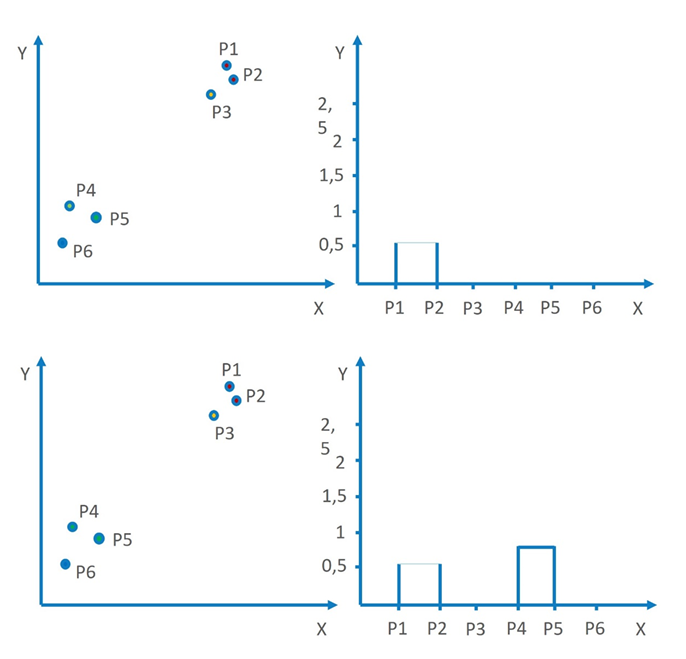
\includegraphics[width=0.5\linewidth]{imagenes/dendrograma1.png}
     \label{fig:dendrograma1}
\end{figure}

\begin{figure}[ht]
     \centering
     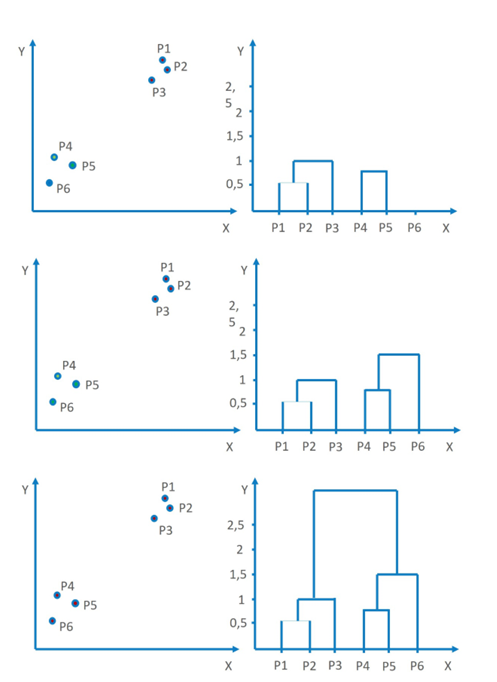
\includegraphics[width=0.5\linewidth]{imagenes/dendrograma2.png}
     \label{fig:dendrograma2}
\end{figure}

\begin{figure}[ht]
     \centering
     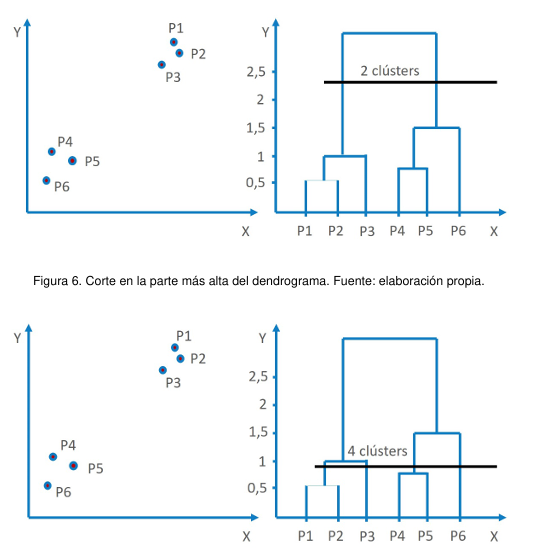
\includegraphics[width=0.5\linewidth]{imagenes/dendrograma3.png}
     \label{fig:dendrograma3}
\end{figure}

\newpage
\section{Distancias de similitud inter-clúster}
Para el ejemplo anterior, el mejor corte es el de 2 clústeres. Debido a que es la distancia más larga y garantiza la suficiente distancia inter-clúster haciendo que cada  grupo este bien diferenciado.

¿Cómo definimos la similitud inter-clúster?
\begin{itemize}
    \item Mínimo o «single linkage algorithm»: es la distancia más corta entre dos puntos que pertenezcan a los dos grupos. Este método puede manejar formas no elípticas. Su limitación es que es altamente sensible a ruido y outliers.

    \item  Máximo o «complete linkage algorithm»: calcula la distancia máxima entre cualquier par de puntos que pertenezcan a diferentes grupos. Es menos susceptible al ruido.

    \item  Media-grupal «average linkage»: calcula la distancia promedio entre todos los pares de puntos de datos que pertenecen a los diferentes grupos. Se obtiene una medida de disimilitud promedio entre grupos. Este método también es menos susceptible al ruido y a los valores atípicos.

    \item Entre-centroides: se calcula el centroide de cada grupo y se calcula la distancia entre ellos.

    \item Método Ward: es una técnica de enlace utilizada en el clustering jerárquico aglomerativo. Su objetivo principal es minimizar la varianza dentro de cada clúster. Cada punto de datos comienza como un clúster individual. En cada paso, se seleccionan los dos clústeres cuya fusión resulta en el menor incremento en la suma total de las varianzas dentro de todos los clústeres. Esta suma se calcula como la suma de las distancias cuadráticas entre cada punto y el centroide del clúster al que pertenece. El proceso de fusión se repite hasta que todos los puntos estén en un solo clúster o se cumpla un criterio de parada específico (por ejemplo, un número
 predefinido de clústeres).
\end{itemize}

\section{K-Means vs Clustering jerárquico}

\begin{figure}[ht]
    \centering
    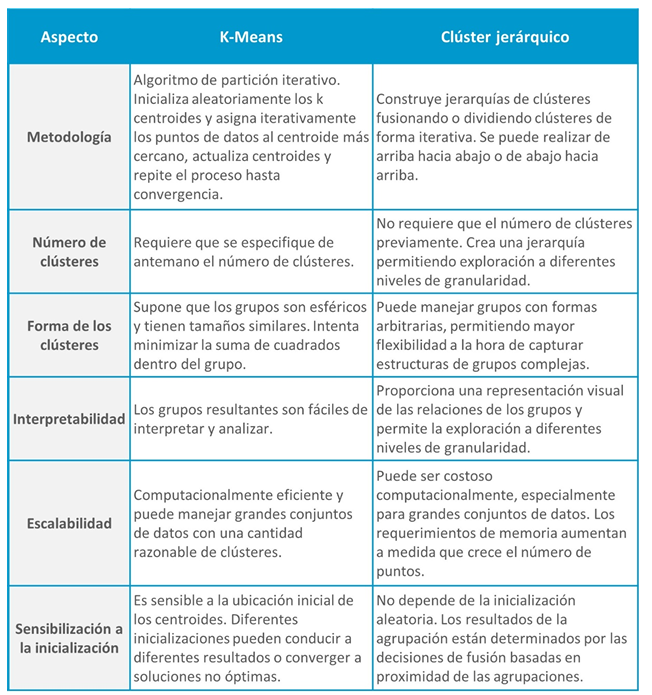
\includegraphics[width=1\linewidth]{imagenes/diferencia-kmeans-clustering-jerarquico.png}
    \label{fig:diferencia-kmeans-clustering-jerarquico}
\end{figure}

\subsection{¿Cuándo usar K-Means y cuándo agrupación jerárquica?}

\begin{itemize}
    \item K-Means funciona muy bien cuando la separación entre los grupos está bien definida. Es eficaz identificando grupos compactos o esféricos; es computacionalmente más eficiente y puede manejar gran cantidad de datos; requiere el número de clústeres previamente;  funciona muy bien con datos numéricos, gracias al manejo de distancias entre puntos; ayuda a crear prototipos y a realizar análisis exploratorio de datos; si tiene una idea de donde se pueden inicializar los clústeres, K-Means puede converger más rápido y producir resultados más precisos.

    \item El clúster jerárquico permite explorar las relaciones dentro de los datos en diferentes niveles de granularidad; es adecuado para conjuntos de datos pequeños o medianos; no requiere que el número de grupos este predeterminado; deal para datos donde existe una estructura jerárquica natural, como taxonomías biológicas, jerarquías organizacionales o relaciones genealógicas; atractivo visual informativo. 
\end{itemize}